\documentclass[11pt]{article}

\usepackage[margin=1in]{geometry}
\usepackage{amsmath,amssymb}
\usepackage{booktabs}
\usepackage{array}
\usepackage{xcolor}
\usepackage{tikz}
\usetikzlibrary{arrows.meta,positioning}
\usepackage{listings}
\usepackage{titlesec}
\usepackage[hidelinks]{hyperref}

\definecolor{acc}{HTML}{C4501E}
\definecolor{boxfill}{HTML}{F4F4F2}
\definecolor{boxline}{HTML}{C9C6C0}
\definecolor{codebg}{HTML}{F7F6F3}

\newcommand{\reg}[1]{\texttt{#1}}
\newcommand{\hx}[1]{\texttt{0x#1}}

\titleformat{\section}{\Large\bfseries\color{black}}{\thesection}{0.6em}{}
\titleformat{\subsection}{\large\bfseries}{\thesubsection}{0.6em}{}

\lstset{basicstyle=\ttfamily\small,backgroundcolor=\color{codebg},
  frame=single,rulecolor=\color{boxline},framesep=6pt,breaklines=true,
  columns=fullflexible,keepspaces=true,xleftmargin=2pt,aboveskip=8pt,belowskip=8pt}

\setlength{\parskip}{4pt}
\setlength{\parindent}{0pt}

\title{\vspace{-1.2cm}\textbf{Lambda KV-Cache Coprocessor}\\[2pt]
\large Micro-Architecture \& Programming Specification}
\author{Longhorn Silicon (Team A71) --- SSCS Chipathon 2026, Track D\\
\texttt{lambda\_kv\_coproc} $\cdot$ GF180MCU core-only macro}
\date{Revision A --- generated from RTL at signoff}

\begin{document}
\maketitle
\vspace{-0.6cm}
\hrule
\vspace{0.5cm}

This document is the practical reference for \emph{talking to} the hardened
\reg{lambda\_kv\_coproc} block over its four-wire SPI link: pinout, clocking, the
byte-level protocol, the address map and data formats, the status/decision
bit-fields, the compress-step state machine, and a complete worked transaction.
All values are taken directly from the RTL as hardened
(\reg{src/lambda\_kv\_coproc.sv}, \reg{src/spi\_loader.sv}); the hardened tile is
$D{=}2,\ L{=}2$.

\tableofcontents
\vspace{0.4cm}
\hrule

\section{Overview and interfaces}
The coprocessor performs one \emph{compress step} per invocation: the host
streams $L$ value tokens ($D$ \texttt{fp16} channels each) and $L$ per-token
attention masses in over SPI; three engines then run and the host reads the
results back. The engines are:
\begin{itemize}\setlength\itemsep{1pt}
\item \textbf{KVE} --- Walsh--Hadamard rotation + per-token amax + INT3
quantization of each value token (codes, scale, reconstruction).
\item \textbf{TIU} --- H2O importance accumulation, a keep-tier bitmap, and a
single eviction victim.
\item \textbf{ACU} --- a divide-free per-tile precision gate.
\end{itemize}

\subsection{Top-level ports}
\begin{center}
\begin{tabular}{@{}lll@{}}
\toprule
Port & Dir & Function \\
\midrule
\reg{clk}       & in  & core clock (see \S\ref{sec:clk}) \\
\reg{rst\_n}    & in  & active-low synchronous-release reset \\
\reg{spi\_sclk} & in  & SPI serial clock (host) \\
\reg{spi\_cs\_n}& in  & SPI frame select, active low \\
\reg{spi\_mosi} & in  & host $\rightarrow$ chip data \\
\reg{spi\_miso} & out\footnotemark & chip $\rightarrow$ host data \\
\reg{obs0..obs3}& out\footnotemark[\value{footnote}] & status taps: busy, done, err, gate\_fp16 \\
\reg{VDD}/\reg{VSS} & pwr & 5\,V core power / common ground \\
\bottomrule
\end{tabular}
\end{center}
\footnotetext{\reg{spi\_miso} and \reg{obs0..obs3} are physically bidirectional
pads (no output-only digital pad exists in the GF180 IO library) used as outputs.}

Build parameters (hardened values): \reg{D=2} (value channels/token, power of
two), \reg{L=2} (cache slots/tokens per step), \reg{ADDR\_WIDTH=16}. Derived
constants below assume these values; where a formula helps, $L$ and $D$ are kept
symbolic.

\subsection{Internal block map}
\begin{center}
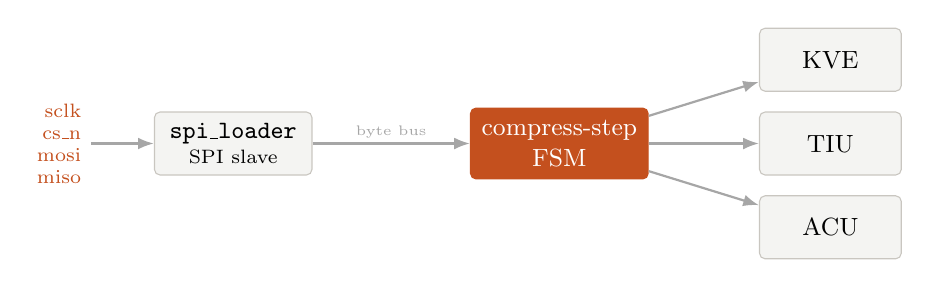
\begin{tikzpicture}[font=\small,
  box/.style={draw=boxline,fill=boxfill,rounded corners=2pt,align=center,
              minimum height=8mm,inner sep=4pt},
  hot/.style={draw=acc,fill=acc,text=white,rounded corners=2pt,align=center,
              minimum height=9mm,inner sep=4pt},
  w/.style={-{Latex[length=2mm]},gray!70,thick}]
  \node[box,minimum width=20mm] (spi) {\reg{spi\_loader}\\[-2pt]\scriptsize SPI slave};
  \node[hot,minimum width=22mm,right=20mm of spi] (fsm) {compress-step\\FSM};
  \node[box,minimum width=18mm,above right=2mm and 14mm of fsm] (kve) {KVE};
  \node[box,minimum width=18mm,right=14mm of fsm] (tiu) {TIU};
  \node[box,minimum width=18mm,below right=2mm and 14mm of fsm] (acu) {ACU};
  \node[left=8mm of spi,align=right,text=acc,font=\scriptsize] (p)
       {sclk\\cs\_n\\mosi\\miso};
  \draw[w] (p) -- (spi);
  \draw[w] (spi) -- node[above,font=\tiny,inner sep=1.5pt]{byte bus} (fsm);
  \draw[w] (fsm) -- (kve); \draw[w] (fsm) -- (tiu); \draw[w] (fsm) -- (acu);
\end{tikzpicture}
\end{center}

The \reg{spi\_loader} decodes SPI frames into a byte-addressed bus
(\reg{bus\_addr}, \reg{bus\_wdata}, \reg{bus\_we}, \reg{bus\_re},
\reg{bus\_rdata}) plus a \reg{start} pulse; it feeds \reg{status\_in} back to the
host. The compress-step FSM owns the buffers and sequences the engines.
Interfaces:
\begin{center}\scriptsize\renewcommand{\arraystretch}{1.25}
\begin{tabular}{@{}>{\raggedright\arraybackslash}p{3.6cm}
                   >{\raggedright\arraybackslash}p{5.3cm}
                   >{\raggedright\arraybackslash}p{5.3cm}@{}}
\toprule
Engine (module) & Inputs from FSM & Outputs to FSM \\
\midrule
KVE\newline\reg{cq\_value\_path\_wht\_syn} & \reg{in\_vec}[$16D$], \reg{dec\_idx} &
  \reg{out\_codes}[$8D$], \reg{out\_scale}, \reg{dec\_rot\_f16} \\
TIU\newline\reg{token\_importance\_unit} & \reg{acc\_*}, \reg{ld\_*},
  \reg{evict\_req}, \reg{tier\_threshold}=48 & \reg{evict\_valid/slot},
  \reg{tier\_keep}, \reg{busy} \\
ACU\newline\reg{precision\_controller} & \reg{s\_valid/data/last} &
  \reg{d\_valid}, \reg{d\_fp16} \\
\bottomrule
\end{tabular}
\end{center}
The KVE is combinational; TIU and ACU are clocked and handshaked by the FSM.

\section{Clocking, reset, and timing budget}
\label{sec:clk}
\textbf{Core clock.} The block is hardened at a \textbf{300\,ns period
($\approx$3.33\,MHz)}; this bound is set by the combinational Walsh--Hadamard
value path and is the maximum core-clock frequency. Timing closes with zero
setup/hold violations at this period.

\textbf{Reset.} \reg{rst\_n} is active low with synchronous release. Hold it low
for several core clocks after power-good; keep \reg{spi\_cs\_n} high (idle) during
reset. On release the FSM is in \reg{S\_IDLE} with all status bits clear.

\textbf{SPI vs.\ core clock (important).} The SPI inputs are \emph{oversampled in
the core clock domain} through a 3-flop synchronizer with rising-edge detection;
there is no dedicated async SPI front end. Correct operation therefore requires
\[
f(\reg{spi\_sclk}) \ll f(\reg{clk}),\qquad
T_{\reg{sclk-phase}} \gtrsim 4\,T_{\reg{clk}} .
\]
In practice budget \textbf{$\ge 8$ core clocks per SPI bit}. With the core at its
3.33\,MHz ceiling this caps \reg{spi\_sclk} at roughly \textbf{400\,kHz}; run
slower (100--250\,kHz) for margin. \reg{spi\_cs\_n} must stay low for the whole
frame and be sampled by at least two core clocks at each edge.

\textbf{At-a-glance status.} Independently of SPI, the observation pins mirror the
status flags live: \reg{obs0}=busy, \reg{obs1}=done, \reg{obs2}=err,
\reg{obs3}=gate\_fp16 --- useful on a logic analyzer or LEDs during bring-up.

\section{SPI protocol}
\textbf{Mode 0 (CPOL=0, CPHA=0), MSB-first.} A frame is delimited by
\reg{spi\_cs\_n} low\,$\rightarrow$\,high. Data changes while \reg{spi\_sclk} is
low and is sampled by the slave on the \emph{rising} edge; the host samples
\reg{spi\_miso} in the high phase. MISO is driven combinationally and is valid
for the whole byte, so the host may sample early in the high phase.

\textbf{Frame layout.}
\begin{center}
\begin{tabular}{@{}cll@{}}
\toprule
Byte & Field & Notes \\
\midrule
0     & \reg{CMD}       & command (below) \\
1     & \reg{ADDR[15:8]} & big-endian address, high byte first \\
2     & \reg{ADDR[7:0]}  & \\
3..n  & \reg{DATA}      & payload; \textbf{address auto-increments per byte} \\
\bottomrule
\end{tabular}
\end{center}

\textbf{Command set.}
\begin{center}
\begin{tabular}{@{}lll@{}}
\toprule
Value & Command & Behaviour \\
\midrule
\hx{01} & \reg{WRITE}  & write \reg{DATA} bytes starting at \reg{ADDR} (auto-inc) \\
\hx{02} & \reg{READ}   & return \reg{DATA} bytes from \reg{ADDR} on MISO (auto-inc) \\
\hx{03} & \reg{START}  & pulse \reg{start}; run one compress step (no \reg{ADDR}/\reg{DATA}) \\
\hx{04} & \reg{STATUS} & MISO returns the STATUS register directly \\
\bottomrule
\end{tabular}
\end{center}

For \reg{READ}, after \reg{CMD}+2 address bytes the host clocks $n$ dummy bytes
(e.g.\ \hx{00}) on MOSI and captures the returned bytes on MISO; the internal
address advances at each byte boundary, so a single frame streams a whole region.
\reg{START} is a one-byte frame. Reading STATUS is normally done with
\reg{READ}~@~\hx{0001} (below); \reg{CMD\_STATUS} is an equivalent shortcut.

\section{Address map and data formats}
16-bit byte address space; multi-byte fields are \textbf{little-endian on the
wire} (low byte first). Element ordering is token-major: token~0's $D$ channels,
then token~1, etc. \reg{fp16} = IEEE half precision.

\begin{center}
\begin{tabular}{@{}llll@{}}
\toprule
Address & Region & Size (bytes) & Dir \\
\midrule
\hx{0300} & \reg{W} --- per-token attention mass (u8) & $L$ & write \\
\hx{0400} & \reg{V} --- value tokens (fp16) & $2LD$ & write \\
\hx{0800} & \reg{CODES} --- rotated INT3 codes (int8) & $LD$ & read \\
\hx{0A00} & \reg{SCALE} --- per-token scale (fp16) & $2L$ & read \\
\hx{0C00} & \reg{VHAT} --- rotated reconstruction (fp16) & $2LD$ & read \\
\hx{0001} & \reg{STATUS} & 1 & read \\
\hx{0002} & \reg{DECISION} & 1 & read \\
\hx{0003} & \reg{KEEP} --- keep-tier bitmap & 1 & read \\
\bottomrule
\end{tabular}
\end{center}

For the hardened tile ($D{=}2,L{=}2$): \reg{W}=2\,B, \reg{V}=8\,B,
\reg{CODES}=4\,B, \reg{SCALE}=4\,B, \reg{VHAT}=8\,B. \reg{V} byte order at
\hx{0400}: token0-ch0 low, token0-ch0 high, token0-ch1 low, token0-ch1 high,
token1-ch0 low, \ldots

\subsection{Status / decision / keep bit-fields}
\reg{STATUS} (\hx{0001}, read-only):
\begin{center}
\begin{tabular}{@{}c|c|c|c|c|c|c|c@{}}
\toprule
bit 7 & 6 & 5 & 4 & 3 & 2 & 1 & 0 \\
\midrule
0 & \reg{err} & \reg{gate\_fp16} & 0 & 0 & 0 & \reg{done} & \reg{busy} \\
\bottomrule
\end{tabular}
\end{center}

\reg{DECISION} (\hx{0002}, read-only):
\begin{center}
\begin{tabular}{@{}c|c@{}}
\toprule
bit 7 & bits $[\,\lceil\log_2 L\rceil{-}1 : 0\,]$ \\
\midrule
\reg{gate\_fp16} & \reg{evict\_slot} \\
\bottomrule
\end{tabular}
\end{center}
For $L{=}2$: bit\,7 = \reg{gate\_fp16}, bit\,0 = \reg{evict\_slot} (bits 6..1 = 0).

\reg{KEEP} (\hx{0003}, read-only): low $L$ bits are the keep-tier bitmap; bit $s$
is set when slot $s$'s accumulated mass $\ge$ \reg{tier\_threshold} (=48). Upper
bits read 0.

\section{Compress-step state machine}
On \reg{START} the FSM leaves \reg{S\_IDLE} (asserting \reg{busy}) and walks the
sequence below, ending in \reg{S\_DONE} (assert \reg{done}, deassert \reg{busy})
and returning to idle. Encodings are the RTL's 4-bit state values.

\begin{center}
\begin{tabular}{@{}clp{9.2cm}@{}}
\toprule
Enc & State & Action \\
\midrule
0 & \reg{S\_IDLE}    & wait for \reg{start}; clear \reg{done}/\reg{err}. \\
1 & \reg{S\_KVE}     & for each token, sweep $D$ channels: latch INT3 code and
  \reg{fp16} reconstruction; capture per-token scale at channel 0. \\
2 & \reg{S\_TIU\_LD} & install $L$ slots into the TIU. \\
3 & \reg{S\_TIU\_ACC}& accumulate each slot's attention mass. \\
4 & \reg{S\_TIU\_EV} & request eviction victim; latch keep-tier bitmap. \\
5 & \reg{S\_PC}      & stream the masses into the ACU as the score tile. \\
6 & \reg{S\_PC\_W}   & wait for the ACU decision; latch \reg{gate\_fp16}. \\
7 & \reg{S\_DONE}    & assert \reg{done}, deassert \reg{busy}; $\rightarrow$ idle. \\
\bottomrule
\end{tabular}
\end{center}

\begin{center}
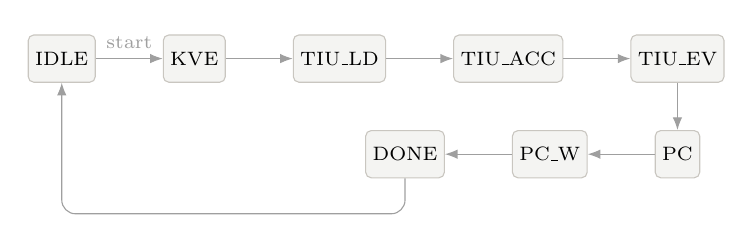
\begin{tikzpicture}[font=\scriptsize,node distance=8.5mm,
  st/.style={draw=boxline,fill=boxfill,rounded corners=2pt,minimum height=6mm,
             inner sep=2.5pt},
  e/.style={-{Latex[length=1.6mm]},gray!75}]
  \node[st] (i)   {IDLE};
  \node[st,right=of i] (k)  {KVE};
  \node[st,right=of k] (l)  {TIU\_LD};
  \node[st,right=of l] (a)  {TIU\_ACC};
  \node[st,right=of a] (v)  {TIU\_EV};
  \node[st,below=6mm of v] (p) {PC};
  \node[st,left=of p]  (pw) {PC\_W};
  \node[st,left=of pw] (d)  {DONE};
  \draw[e] (i)--node[above]{start} (k);
  \draw[e] (k)--(l); \draw[e] (l)--(a); \draw[e] (a)--(v);
  \draw[e] (v)--(p); \draw[e] (p)--(pw); \draw[e] (pw)--(d);
  \draw[e,rounded corners=5pt] (d.south) -- ++(0,-4.5mm) -| (i.south);
\end{tikzpicture}
\end{center}

\textbf{Error / timeout.} \reg{S\_TIU\_EV} bounds the eviction handshake and
proceeds even if it times out. \reg{S\_PC\_W} bounds the ACU handshake; if the
decision does not arrive within its window it sets \reg{err} (STATUS bit\,6) and
goes to \reg{S\_DONE}. A run with \reg{err}=1 means the ACU did not respond;
\reg{done} still asserts so the host's poll terminates.

\section{Address decode}
All decode is combinational in the coprocessor:
\begin{itemize}\setlength\itemsep{1pt}
\item \textbf{Write:} \reg{bus\_we} writes \reg{W} when
\reg{bus\_addr}$\in[\hx{0300},\hx{0300}{+}L)$ and \reg{V} when
$\in[\hx{0400},\hx{0400}{+}2LD)$; for \reg{V} the low address bit selects the
low/high \reg{fp16} byte.
\item \textbf{Read mux:} \hx{0001}$\to$STATUS, \hx{0002}$\to$DECISION,
\hx{0003}$\to$KEEP, \reg{CODES}/\reg{SCALE}/\reg{VHAT} from their windows; any
other address reads \hx{00}.
\end{itemize}

\section{Programming sequence (worked example)}
One full compress step for $D{=}2,L{=}2$. Each line is one SPI frame
(\reg{CS} low $\ldots$ high). Bytes are hex; \reg{--} marks captured MISO bytes.

\begin{lstlisting}
; 1. write attention masses W (2 bytes) at 0x0300
WRITE 0x0300  m0 m1                       ; CMD=01 ADRH=03 ADRL=00 DATA=m0,m1

; 2. write value tokens V (fp16 LE, 8 bytes) at 0x0400
WRITE 0x0400  t0c0L t0c0H t0c1L t0c1H
              t1c0L t1c0H t1c1L t1c1H

; 3. kick one compress step
START                                     ; CMD=03 (no address/data)

; 4. poll STATUS until done (bit1), bounded; check err (bit6)==0
loop: READ 0x0001 -> s                    ; CMD=02 ADRH=00 ADRL=01, 1 dummy byte
      until (s & 0x02)                     ; done
      assert (s & 0x40) == 0               ; err clear

; 5. read the decision + keep bitmap
READ 0x0002 -> d      ; bit7=gate_fp16, bit0=evict_slot (L=2)
READ 0x0003 -> keep   ; bits[1:0] = keep-tier per slot

; 6. read the compressed records
READ 0x0800 -> c0 c1 c2 c3                 ; CODES  (L*D = 4 int8, range [-4,3])
READ 0x0A00 -> s0L s0H s1L s1H             ; SCALE  (L fp16)
READ 0x0C00 -> h0L h0H ... h3L h3H         ; VHAT   (L*D fp16)
\end{lstlisting}

A \reg{READ} frame sends \reg{CMD=02}, the two address bytes, then $n$ dummy MOSI
bytes while capturing $n$ MISO bytes; the address auto-increments, so the whole
region streams in one frame.

\section{Caveats and known issues}
\begin{itemize}\setlength\itemsep{2pt}
\item \textbf{Reserved low addresses \hx{0000}--\hx{0005}.} The loader keeps
vestigial local CSR shadows here from an earlier datapath. A \reg{WRITE} to
\hx{0000} pulses \reg{start} (bit\,0) and latches \reg{precision\_sel}
(bits\,[2:1]); writes to \hx{0002}--\hx{0005} land in unused local registers.
\textbf{Do not write \hx{0000}--\hx{0005}}; use \reg{CMD\_START} to start.
(Reads at \hx{0001}/\hx{0002}/\hx{0003} return the coprocessor STATUS/DECISION/
KEEP as documented.)
\item \textbf{Loader front end.} The SPI slave oversamples in the core domain and
is documented in-RTL as a pre-tapeout skeleton (no metastability-hardened async
front end). Respect the \reg{spi\_sclk} $\ll$ \reg{clk} budget of \S\ref{sec:clk}.
\item \textbf{Scope.} Verified at the RTL + physical-signoff level (self-checking
SPI test + LVS). No gate-level sim; the SPI test is a targeted deterministic
check, not exhaustive coverage. See \reg{docs/VERIFICATION.md}.
\end{itemize}

\vspace{0.3cm}
\hrule
\vspace{0.2cm}
{\footnotesize\raggedright Source of truth: \reg{src/lambda\_kv\_coproc.sv},
\reg{src/spi\_loader.sv} on \texttt{main}. Functional model:
\reg{src/tb\_coproc\_spi.sv} (\reg{make sim-coproc}).\par}

\end{document}
